\chapter{Проектирование и применение модульного технологического оборудования}\label{ch:ch2}

\paragraph{Принципы унификации оборудования.}

Проблема унификации оборудования стоит особняком в ряду проблем, возникающих в области стандартизации. На сегодняшний день унификация распространена повсеместно и включает в себя самые разные нормы, требования, процессы, методы и документы. Однако потребность в решении проблемы унификации по-прежнему существует. Данное утверждение подтверждается действующими нормативными документами. В данных нормативных документах регламентируются такие параметры, как номенклатура и содержание основных требований, предъявляемых к унификации, состав и структура проводимых работ по унификации и т.\,д. К сожалению, данные стандарты в первую очередь направлены на военно-промышленный комплекс, где вопросам стандартизации и унификации уделяется особое внимание. Поэтому на сегодняшний день можно постулировать, что проблемы общепромышелнной унификации и дальнейшее совершенствование теоретических основ унификации остаются крайне актуальными для нашей страны. 

Сейчас в промышленном производстве унификация практически забыта. Последнее обуславливается множеством факторов, к которым можно отнести несовершенное нормативно-правовое обеспечение и недостаточную научную проработанность унификации с точки зрения современного промышленного производства. Из значимых работ есть только учебные издания, которые описывают зачастую уже устаревшие нормы и правила. 

Безусловно, причиной недостаточно развития принципов унификации в нашей стране можно назвать отказ от плановой экономики и возникающих вследствие этого недочетов в управлении отдельными предприятиями, работающими по принципа рыночной экономики. Очевидно, что основная цель таких предприятий сиюминутная прибыль, при это решение более важных и перспективных в плане ценности конечного результата задач по большей части откладывается на неопределенный срок. 

Поэтому в настоящее время практически не появляются какие-либо индустриальные стандарты производства высокотехнологичной продукции. На первое место выходит защита собственных интеллектуальных интересов, а потенциальная выгода от работы в коллаборации с конкурентами представляется чем-то недостижимым. Конечно, решающую роль в формировании подобных отраслевых стандартов должно играть государство, но в рамках рыночной экономики открытым остается вопрос применимости стандартов <<навязанных>> сверху. Исходя из всего вышесказанного можно выделить следующие основные причины пренебрежения принципами унификации на современных предпритяиях:

\begin{itemize}
	\item отсутствие какой-то экономической заинтересованности во внедрении унифицированных составных частей в своих изделиях, если эти изделия разработаны другими предприятиями (хотя такие прецеденты существуют);
	\item отсутствие практики конкурсных разработок важных составных частей и изделий (за исключением работы в пользу государственных/оборонных предприятий);
	\item отсутствие четкой информация по унифицированным и стандартизованным составным частям распространенных изделий.
\end{itemize}

Учитывая вышесказанное, задача унификации модулей и шасси модульного технологического оборудования стоит достаточно остро. В то время как унификация немодульного оборудования важна в большей степени производителю, чтобы удешевить производство, обслуживание и ремонт, унификация модульного оборудования в значительной мере касается и потребителя. Унификация модулей и шасси позволят с одной стороны сократить их многообразие, а с другой увеличить количество возможных собираемых конфигураций. 

Основными инструментами унификации являются параметрические ряды и ограничения. Для составления параметрических рядов есть ряд правил, закрепленных в соответствующих нормативных документах.\footnote{ГОСТ 23945.0-80. Унификация изделий. Основные положения}\footnote{РД 50-632-87 Методические указания. Унификация изделий построение параметрических и типоразмерных рядов деталей и сборочных единиц общемашиностроительного применения} Обычно параметрические ряды составляются из некоторого ряда предпочтительных чисел,\footnote{ГОСТ 8032-84. Предпочтительные числа и ряды предпочтительных чисел} представляющего собой числовую последовательность, полученную по определенному правилу, например, правилу арифметической или геометрической прогрессии.

\paragraph{Особенности конструкции модулей.}

Несомненно, модули могут различаться по размеру в зависимости от решаемой задачи. Причем, в соответствии с принципом унификации, система управления должна определять положение подключенного модуля самостоятельно и без необходимости ручной настройки или калибровки. Известно, что точность обработки зависит от точности взаимного геометрического положения всех компонентов промышленного оборудования. Этого чрезвычайно сложно достичь при применении модульного подхода, поскольку положение модуля относительно системы координат шасси заранее неизвестно.

Более высокую точность позиционирования можно получить, изменив способ установки модулей на подвеске каретки и, например, используя крепления <<ласточкин хвост>> с клиновым зажимом. Описанная схема широко применяется в быстросменных резцедержателях металлообрабатывающих станков. Такой подход обеспечивает отличную точность и повторяемость при переустановке модулей вручную. Однако это значительно усложняет общую конструкцию подвеса каретки из-за необходимости высокоточной обработки сопрягаемых деталей (требуется шлифование всех сопрягаемых поверхностей в соединении), а также увеличивается общий вес подвижной части в системе. Кроме того, все модули должны иметь одинаковые ответные части типа <<ласточкин хвост>>, размеры которых зависят не от размера самого модуля, а от размеров шасси. Следовательно, нарушается принцип универсальности, поскольку в этом случае невозможно установить малогабаритный модуль на большое шасси.

Усилия используемых в настоящее время магнитных крепления вполне достаточно для установки практически всех видов измерительных и обрабатывающих модулей. Однако, все эксперименты с обработкой металлов проводились на маломощных шпинделях при небольшой глубине резания. Последнее обусловлено небольшими габаритами и жесткостью экспериментальной установки. Однако, как уже отмечалось ранее, предполагается разработка линейки трехкоординатных платформ разного размера и жесткости. Очевидно, что для более габаритных платформ будут использоваться более тяжелые режимы обработки резанием, при которых возможен отрыв шпиндельного модуля от посадочной поверхности подвеса каретки. Данная проблема требует дополнительных исследований.

Наиболее целесообразным представляется использование электромагнитов вместо постоянных магнитов. Данное предположение подтверждается наличием на рынке специализированных сверлильных станков на магнитной подошве.\footnote{Электронный ресурс: {\tiny\url{https://www.bds-machines.com/magnetic-drilling-machines/mab-825-kts/}} (дата обращения: 20.09.2019).} С их помощью осуществляется сверление, рассверливание, зенкерование, нарезания резьбы даже фрезерование в различных металлоконструкциях в судостроении, тяжёлом машиностроении, при ремонте трубопроводов, при выполнении строительных работ и т. д. Широкое распространение подобных станков связано с применением современных электромагнитных плит с большой удерживающей силой, являющихся основанием станков. Данный положительный опыт может быть использован для модернизации предлагаемой концепции установки модулей.

Также стоит отметить, что одним из вариантов использования модульного оборудования является включение его в гибкие производственные линии, где потребуется автоматическая замена модуля с использованием промышленного робота-манипулятора. Анализ современного оборудования показал, что достаточное усилие прижатия клинового зажима может быть достигнуто только с помощью пневматических зажимов. Это приводит к необходимости дополнительной воздушной линии, что также усложняет первоначальный предложенный подход.

Вместо этого предлагается использовать магнитную систему крепления с дополнительной направляющей канавкой, расположенной в плоскости, параллельной направлению каретки~(рисунок~\cref{fig:quick-mount}). Описанная система крепления позволяет использовать модули любого размера; однако возникает проблема объединения систем координат модуля и основного шасси. В данной работе предлагается комбинированная система автоматического позиционирования модуля на подвеске каретки с использованием машинного зрения. Эта система определяет расположение специализированных оптических маркеров на шасси и автоматически изменяет геометрические параметры, используемые в системе управления.

\begin{figure}[ht]
	\centerfloat{
		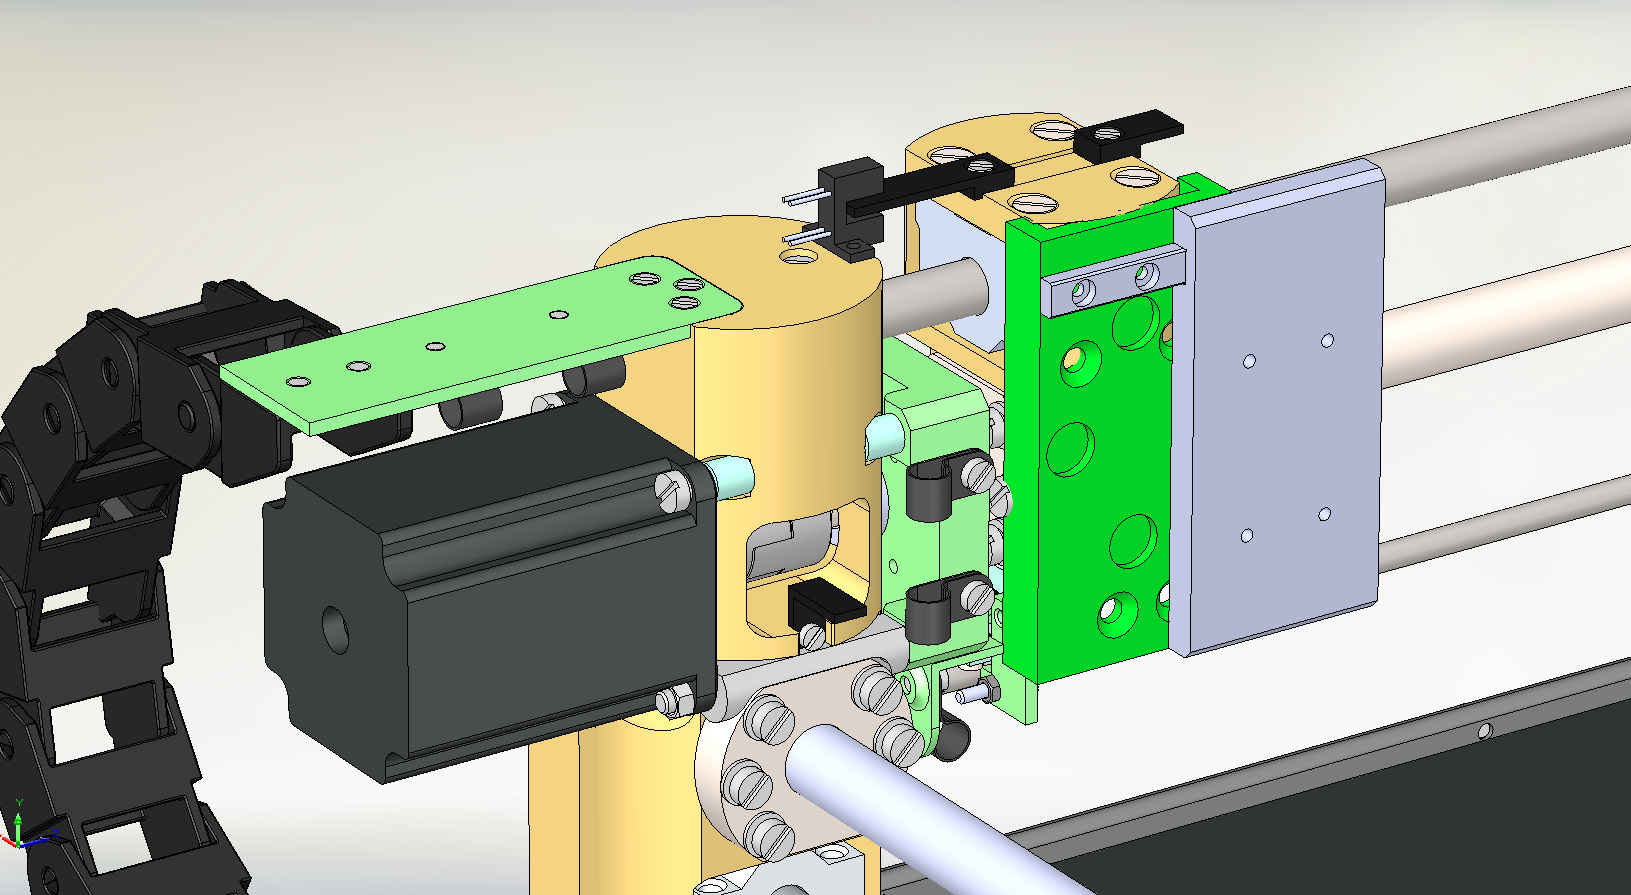
\includegraphics[width=0.9\textwidth]{ch-2/quick-mount.png}
	}
	\caption{Конструкция магнитного крепления модуля}\label{fig:quick-mount}
\end{figure}

\paragraph{Этапы унификации модульного оборудования}

Первым этапом является определение параметров подлежащих унификации. Для модулей с электромагнитным креплением основными параметрами будут:

\begin{itemize}
	\item Грузоподъемность электромагнита.\footnote{сноска главный параметр}
	\item Ширина присоединительной поверхности модуля. 
	\item Глубина модуля.
	\item Ток потребления модуля.
\end{itemize}

-- картинка --

Из данного списка необходимо выбрать главный параметр. Обычно главный параметр выбирают как параметр наиболее полно характеризующий несущую способность или другую эксплуатационную характеристику. Поскольку модули имеют различную функциональность, то в качестве главного параметра выбрана грузоподъемность электромагнита, характеризующая выдерживаемое усилие. Этот параметр с одной стороны косвенно связан с массой модуля, а соответственно возможностью его установки на каретку того или иного шасси. С другой стороны он может быть связан с технологическими режимами работы модуля, например с силой резания при фрезеровании. В качестве фиксированных параметров приняты:

\begin{itemize}
	\item Напряжение питания.
	\item Параметры ответной части паза.
\end{itemize}

Напряжение питания выбрано в качестве фиксированного параметра, чтобы избежать применения преобразователей напряжения и использовать напряжение 24В де-факто ставшее промышленным стандартом. Параметры ответной части паза должны быть зафиксированы для обеспечения  широких возможностей по установки нескольких модулей одновременно. Следующим этапом необходимо определить ограничения выбранных параметров. Для модулей с электромагнитным креплением было выявлено пять ограничений.

\paragraph{Ограничение массы модуля в зависимости от грузоподъемности электромагнита.} При проектировании модуля необходимо учитывать его суммарную массу. Вес модуля должен быть меньше отрывного усилия в $1/(1-k)$ раз. Где $k$ "--- это коэффициент запаса. Формально ограничение может быть описано как:

-- формула --

При этом, если предполагается устанавливать данный модуль одновременно с другими, то ограничение приобретает вид:

-- формула --

\paragraph{Ограничение грузоподъемности электромагнита в зависимости грузоподъемности шасси.} При проектировании модуля необходимо учитывать что грузоподъемность электромагнита, а соответственно максимально устанавливаемая на шасси масса (масса модуля), должна была меньше грузоподъемности шасси c учетом коэффициента запаса.

-- формула --

Ограничение тока потребления модуля в зависимости от максимального рабочего тока шасси. Ток потребления модуля должен быть меньше рабочего тока шасси c учетом коэффициента запаса.

-- формула --

Если предполагается устанавливать данный модуль одновременно с другими, то:

-- формула --

\paragraph{Ограничение глубины модуля в зависимости от рабочего пространства.} Глубина модуля определяет доступное рабочее пространство шасси в зависимости от общего рабочего поля шасси. С увеличением глубины модуля для обеспечение заданного рабочего пространства модуля необходимо увеличивать общее рабочее поля шасси. Тогда ограничение может быть записано как:

--формула--

Если предполагается устанавливать данный модуль одновременно с другими, то:

--формула--

\paragraph{Ограничение на ширину присоединительной поверхности модуля.} Необходимо обеспечить возможность уместить модуль совместно с N-1 другими модулями компактно. Где критерий компактности это:

--формула--

Последним этапом необходимо сформировать параметрические ряды. Для параметра грузоподъемности электромагнита можно использовать ряд предпочтительных чисел, при этом ряд должен быть ограничен сверху грузоподъемностью шасси.
--формула--

Параметрический ряд глубины модуля можно также сформировать из ряда предпочтительных чисел, при этом ряд должен быть ограничен сверху величиной равной разнице  рабочее поле шасси - минимальное желаемое рабочего поле модуля.

--формула--

Параметр ширины присоединительной поверхности не может быть выбран из  ряда предпочтительных чисел, поскольку это не гарантирует обеспечения компактности. Тогда, исходя из критерия компактности можно синтезировать кратные ряды вида 

--формула--

Используя инструментарий полученных параметрических рядов, проектировщик модулей может добиться совместимости разрабатываемого модуля с шасси и модулями других разработчиков, при это не имея описания и документации на объекты совместимости. Кроме этого возможно достижение опережающей совместимости с объектами разработанными в будущем. Более того, появляется возможность на основе полученного формального описания рядов создать автоматизированную систему расчета параметров и проверки совместимости.

%-----------------------------------------------------------------------------------------------------------------------------------------------

\section{Математическая модель унификации, параметризации и оптимизации компонентов модульной технологической платформы}

\section{Модель оптимизации модульного оборудования при единичном и мелкосерийном производствах}

Рассмотрим основные понятия оптимизации по номенклатуре выпускаемых изделий. Пусть $N$ "--- номенклатура групп изделий, предлагаемая для выпуска, полученная на этапе маркетинговых исследований:

\[
N = {D_1, D_2, \ldots, D_i}, N = (D_i)_{i \in I},
\]

\noindent где $D_i$ "--- группа изделий. Группирование происходит по технологическому признаку [Митрофанов, стр. 43] "--- \textit{вид обработки}.

\[
D = {P_1, P_2, \ldots, P_j},
\]

\noindent где $P_j$ "--- групповая технологическая операция. В соответствие каждой группе ставится вероятность спроса:

\[
f: D_i \rightarrow \upsilon_i, D_i \in N, \upsilon_i \in V,
\]

\noindent где $V$ "--- множество вероятностей такое, что:

\[
\forall\upsilon\in V: \upsilon\leq 1 \wedge\upsilon > 0
\]

Определим композицию для нахождения наиболее вероятной группы или нескольких групп:

\[
g: V \rightarrow N', \forall\upsilon = V_max: \upsilon \in f(N'), V_max \in V, N' \subset N
f \circ g = h,
\]

\noindent где $N' = (D_j)_{j \in J}$ "--- результат композиции (семейство наиболее вероятных групп), $\bigcup N' = {p:p_1\in D_1 \vee p_2\in D_2 \vee\ldots\vee p_j\in D_j}$ "--- множество групповых операций в этих группах.

Фактическая номенклатура задаётся нечётким множеством:

\[
N'' = {(D, \upsilon(D)) \mid D \in N}
\]

Определить коэффициенты целесообразности использования модульности можно как:

\[
\epsilon = \frac{\big|\bigcup N' \big|}{|G|},
\]

\noindent где $G$ "--- домен операций, $\bigcup\limits_{i} N$. Если $\epsilon\rightarrow 0$ "--- модульность целесообразна, если $\epsilon\rightarrow 1$ "--- модульность нецелесообразна.

\section{Определение критерия оптимизации конфигурации модульного оборудования}

\section{Разработка параметрического ряда ширины присоединительной поверхности}



\section{Выводы по главе 2}


\FloatBarrier